% !TeX program = xelatex
% Build from this directory: xelatex defense_slides; bibtex defense_slides;
% xelatex defense_slides; xelatex defense_slides. Use -output-directory to
% isolate artifacts during concurrent thesis builds. No seminar file is input.
% Read before composition: completed thesis introduction, preliminaries,
% literature, geometry, method, results, conclusions, appendix, research.bib.
% 30 main frames, approximately 27 minutes; backups follow the appendix.
% All empirical evidence is from the joint SORA paper, not new experiments.
\documentclass[11pt,aspectratio=169,professionalfonts]{beamer}
\usetheme{Madrid}
\usecolortheme{whale}
\usepackage{amsmath,amssymb,booktabs,array,graphicx}
\usepackage{tikz}
\usetikzlibrary{arrows.meta,positioning}
\usepackage{appendixnumberbeamer}
\usepackage{xepersian} % LAST package: bidi must see all previous packages.

\IfFileExists{../../Master's Thesis - Farzan Rahmani/v2/styles/fonts/XB Niloofar.ttf}{%
  \settextfont[Path={../../Master's Thesis - Farzan Rahmani/v2/styles/fonts/},
    BoldFont={XB NiloofarBd.ttf},ItalicFont={XB NiloofarIt.ttf},
    BoldItalicFont={XB NiloofarBdIt.ttf}]{XB Niloofar.ttf}
  \newfontfamily\persiansans[Script=Arabic,
    Path={../../Master's Thesis - Farzan Rahmani/v2/styles/fonts/},
    BoldFont={XB NiloofarBd.ttf},ItalicFont={XB NiloofarIt.ttf},
    BoldItalicFont={XB NiloofarBdIt.ttf}]{XB Niloofar.ttf}
}{%
  \IfFontExistsTF{Vazirmatn}{\settextfont{Vazirmatn}
    \newfontfamily\persiansans[Script=Arabic]{Vazirmatn}}{%
    \settextfont{Tahoma}\newfontfamily\persiansans[Script=Arabic]{Tahoma}}
}
\setlatintextfont{TeX Gyre Termes}
\setlatinsansfont{TeX Gyre Termes}
% Beamer selects sans; explicitly restore the Persian family for every frame.
\renewcommand{\sfdefault}{\rmdefault}
\setbeamerfont{normal text}{family=\persiansans,size=\fontsize{14}{19}}
\setbeamerfont{frametitle}{family=\persiansans,size=\fontsize{19}{24},series=\bfseries}
\setbeamerfont{block title}{family=\persiansans,size=\normalsize,series=\bfseries}
\setbeamerfont{caption}{size=\fontsize{10}{13}}
\setbeamerfont{footnote}{size=\fontsize{9}{11}}
\AtBeginEnvironment{frame}{\persiansans\fontsize{14}{19}\selectfont}
\graphicspath{{./images/}}
\definecolor{sharifblue}{RGB}{0,51,102}
\definecolor{accent}{RGB}{0,121,140}
\setbeamercolor{structure}{fg=sharifblue}
\setbeamercolor{title}{fg=white,bg=sharifblue}
\setbeamercolor{frametitle}{fg=white,bg=sharifblue}
\setbeamercolor{palette primary}{fg=white,bg=sharifblue}
\setbeamercolor{palette secondary}{fg=white,bg=sharifblue!80}
\setbeamercolor{palette tertiary}{fg=white,bg=sharifblue!60}
\setbeamercolor{block title}{fg=white,bg=sharifblue}
\setbeamercolor{block body}{fg=black,bg=sharifblue!5}
\setbeamercolor{alerted text}{fg=accent}
\setbeamersize{text margin left=8mm,text margin right=8mm}
\setbeamertemplate{navigation symbols}{}
\setbeamertemplate{headline}{}
\setbeamertemplate{caption}{\raggedleft\insertcaption\par}
\setbeamertemplate{itemize item}{\color{accent}\textbullet}
\setbeamertemplate{bibliography item}[text]
\setbeamertemplate{footline}{%
  \leavevmode\hbox{%
    \begin{beamercolorbox}[wd=.27\paperwidth,ht=3ex,dp=2ex,center]{author in head/foot}
      \persiansans\fontsize{9}{10}\selectfont فرزان رحمانی
    \end{beamercolorbox}%
    \begin{beamercolorbox}[wd=.57\paperwidth,ht=3ex,dp=2ex,center]{title in head/foot}
      \persiansans\fontsize{9}{10}\selectfont دفاع کارشناسی ارشد | آموزش هم‌آورد سریع
    \end{beamercolorbox}%
    \begin{beamercolorbox}[wd=.16\paperwidth,ht=3ex,dp=2ex,center]{date in head/foot}
      \fontsize{9}{10}\selectfont\lr{\insertframenumber\,/\,\inserttotalframenumber}
    \end{beamercolorbox}}}
% Original seminar branding/logo; logo is an institutional mark, not a result figure.
\logo{
\includegraphics[height=5mm]{logo.pdf}\hspace{1mm}}
\setbeameroption{hide notes} % Default PDF contains slides only.
% For presenter output, change the preceding option to show notes.
\newcommand{\src}[1]{\par\vspace{1mm}{\fontsize{9}{11}\selectfont\color{sharifblue}#1\par}}
\newcommand{\takeaway}[1]{\begin{block}{پیام اصلی}#1\end{block}}
\newcommand{\sora}{\lr{SORA}}
\newcommand{\pa}{\lr{PertAlign}}
\DeclareMathOperator{\sign}{sign}
\title{پیش‌بینی بیش‌برازش فاجعه‌بار در آموزش تخاصمی سریع}
\author{فرزان رحمانی}
\institute{دانشگاه صنعتی شریف؛ دانشکدهٔ مهندسی کامپیوتر}
\date{} % No date or committee was supplied.
\hypersetup{pdftitle={پیش‌بینی بیش‌برازش فاجعه‌بار در آموزش تخاصمی سریع},
  pdfauthor={Farzan Rahmani},pdfsubject={MSc Defense; SORA}}

\begin{document}

% MAIN 01 | 0:40
\begin{frame}[plain]
\centering

\includegraphics[height=13mm]{logo.pdf}\par
{\fontsize{12}{16}\selectfont دانشگاه صنعتی شریف | دانشکدهٔ مهندسی کامپیوتر\par}
{\fontsize{12}{16}\selectfont دفاع پایان‌نامهٔ کارشناسی ارشد هوش مصنوعی و رباتیک\par}
\vspace{4mm}
\begin{beamercolorbox}[wd=\textwidth,sep=3mm,center,rounded=true]{title}
{\fontsize{21}{29}\selectfont\bfseries پیش‌بینی بیش‌برازش فاجعه‌بار\\ در آموزش تخاصمی سریع\par}
\end{beamercolorbox}
\vspace{4mm}
فرزان رحمانی \quad | \quad شمارهٔ دانشجویی: \lr{403210725}\par
استاد راهنما: دکتر محمدحسین رهبان
\note{زمان هدف: حدود ۲۷ دقیقه. عنوان پیشنهاد اولیه با واژهٔ تخاصمی حفظ شده است؛ در ادامه مطابق واژه‌نامهٔ پایان‌نامه از هم‌آورد استفاده می‌کنم. هدف، پیش‌بینی کم‌هزینهٔ شکست آموزش تک‌گامی و پیوند آن با اصلاح گام است.}
\end{frame}

% MAIN 02 | 0:40
\begin{frame}{مسیر دفاع: از مشاهدهٔ شکست تا کنترل گام}
\begin{enumerate}
\item مسئله: چرا درستی زیادِ تک‌گامی می‌تواند گمراه‌کننده باشد؟
\item تحلیل و روش: هندسهٔ هزینه، \pa{} و کنترل‌کنندهٔ \sora.
\item شواهد: ستبری، انتقال تنظیمات، هزینه و حدود اعتبار.
\end{enumerate}
\src{مبنای علمی: مقالهٔ مشترک \sora{} در \lr{ICML 2026} \cite{sora2026}؛ فصل‌های ۱ تا ۷ و پیوست پایان‌نامه.}
\note{مقالهٔ مشترک به ترتیب نوشتهٔ مزدک تیموریان، رامتین مسلمی، فرزان رحمانی و محمدحسین رهبان است. اعداد و نمودارها از مقاله‌اند؛ در تدوین پایان‌نامه آزمایش تازه‌ای اجرا نشده است. حدود ۶ دقیقه مسئله، ۱۳ دقیقه تحلیل و روش، و ۸ دقیقه شواهد و جمع‌بندی.}
\end{frame}

% MAIN 03 | 0:50
\begin{frame}{پرسش عملی و مدل تهدید}
\begin{itemize}
\item می‌خواهیم شکست تقریب تک‌گامی را با اطلاعات موجود آموزش زودتر ببینیم و اصلاح کنیم.
\item مهاجمِ بدون هدف و جعبه‌سفید، هزینهٔ دسته‌بندی تصویر را افزایش می‌دهد.
\item معیار، درستی تجربی در برابر حملهٔ قوی است؛ گواهی ریاضی ستبری نیست.
\end{itemize}
\[
\Delta_\infty(x,\epsilon)=\{\delta:\|\delta\|_\infty\leq\epsilon,
\quad x+\delta\in[0,1]^d\}
\]
\src{مبانی مدل تهدید و ارزیابی: \cite{madry2018towards,croce2020reliable}.}
\end{frame}

% MAIN 04 | 0:50
\begin{frame}{آموزش هم‌آورد: دو مسئلهٔ درهم‌تنیده}
\[
\min_\theta\;\mathbb E_{(x,y)\sim\mathcal D}
\left[\max_{\delta\in\Delta_\infty(x,\epsilon)}
\mathcal L(f_\theta(x+\delta),y)\right]
\]
\begin{itemize}
\item مسئلهٔ درونی: یافتن نمونه‌ای با هزینهٔ زیاد برای مدل فعلی.
\item مسئلهٔ بیرونی: به‌روزرسانی وزن‌ها روی همان نمونه.
\item آموزش سریع هزینهٔ حل درونی را کم می‌کند؛ کیفیت این تقریب باید پایش شود.
\end{itemize}
\src{صورت‌بندی: \cite{madry2018towards}؛ آموزش سریع: \cite{wong2020fast}.}
\end{frame}

% MAIN 05 | 1:00
\begin{frame}{یک شیب در برابر بازبینی چندبارهٔ جهت}
\textbf{حملهٔ علامت شیب سریع؛ تقریب مرتبهٔ اول:}
\[
g=\nabla_x\ell(x),\qquad
x_{\mathrm{FGSM}}=\Pi_{[0,1]^d}(x+\epsilon\sign(g))
\]
\textbf{حملهٔ چندگامی با تصویرشدن؛ \lr{PGD}:}
\[
\delta^{t+1}=\Pi_{\Delta_\infty(x,\epsilon)}
\left(\delta^t+a\sign\bigl(\nabla_x\ell(x+\delta^t)\bigr)\right)
\]
\begin{itemize}
\item \lr{FGSM} جهت آغاز را ثابت نگه می‌دارد؛ \lr{PGD} تغییر جهت را می‌بیند.
\item بودجهٔ $\epsilon$ و اندازهٔ گام $a$ دو کمیت متفاوت‌اند.
\end{itemize}
\src{\lr{FGSM}: \cite{goodfellow2015explaining}؛ \lr{PGD}: \cite{madry2018towards}.}
\end{frame}

% MAIN 06 | 0:45
\begin{frame}{بیش‌برازش فاجعه‌بار: موفقیت ظاهریِ حل‌کننده}
\begin{itemize}
\item درستی زیر حملهٔ چندگامی در زمانی کوتاه فرو می‌ریزد.
\item درستی زیر حملهٔ تک‌گامی آموزش ممکن است همچنان زیاد بماند.
\item هزینهٔ کم در انتهای حمله، بیشینهٔ هزینه در همسایگی را تضمین نمی‌کند.
\end{itemize}
\takeaway{باید اعتبار مولد نمونهٔ آموزشی را بسنجیم؛ ارزیابی با همان حملهٔ آموزش کافی نیست.}
\src{تعریف و تحلیل پدیده: \cite{wong2020fast,andriushchenko2020understanding}.}
\note{این پدیده با افت تدریجی تعمیم ستبر یکی نیست. مدل می‌تواند نقاطی را که مولد ضعیف به آن‌ها می‌رسد ترمیم کند، درحالی‌که نقاط پرهزینهٔ میان راه باقی می‌مانند.}
\end{frame}

% MAIN 07 | 1:10
\begin{frame}{روش‌های پیشین چه چیزی را تغییر می‌دهند؟}
% Provenance: newly composed qualitative table from paper SORA Sec.2 and
% thesis literature; NOT an original paper/seminar table or new experiment.
\begin{table}
\centering\fontsize{12}{16}\selectfont
\renewcommand{\arraystretch}{1.25}
\begin{tabular}{p{.20\linewidth}p{.31\linewidth}>{\raggedleft\arraybackslash}p{.36\linewidth}}
\toprule
خانواده & نمونه & سازوکار و پرسش باز \\
\midrule
تنوع آشفتگی & \lr{FGSM-RS, N-FGSM} & تنوع آغاز و دامنه؛ انتقال تنظیمات؟ \\
منظم‌سازی & \lr{GradAlign, NuAT, ELLE} & کنترل هندسه؛ هزینهٔ محاسبات؟ \\
نمونهٔ غیرعادی & \lr{AAER} & کنترل افت هزینه؛ زمان ظهور نشانه؟ \\
گام تطبیقی & \lr{ATAS} & استفاده از بزرگی شیب؛ اطلاعات خمیدگی؟ \\
\bottomrule
\end{tabular}
\caption{تدوین تازه از مرور بخش ۲ مقالهٔ \sora{} \cite{sora2026}؛ این جدول در اصل مقاله یا سمینار وجود ندارد.}
\end{table}
\src{منابع روش‌ها: \cite{dejorge2022make,andriushchenko2020understanding,sriramanan2021towards,rocamora2024efficient,lin2023eliminating,huang2023fast}.}
\end{frame}

% MAIN 08 | 0:55
\begin{frame}{هندسه: یک گام می‌تواند از ناحیهٔ آسیب‌پذیر عبور کند}
% Provenance: supplied paper_geometry.pdf, published SORA Figure 1;
% original paper figure, reproduced unchanged, not seminar/new evidence.
\begin{figure}
\centering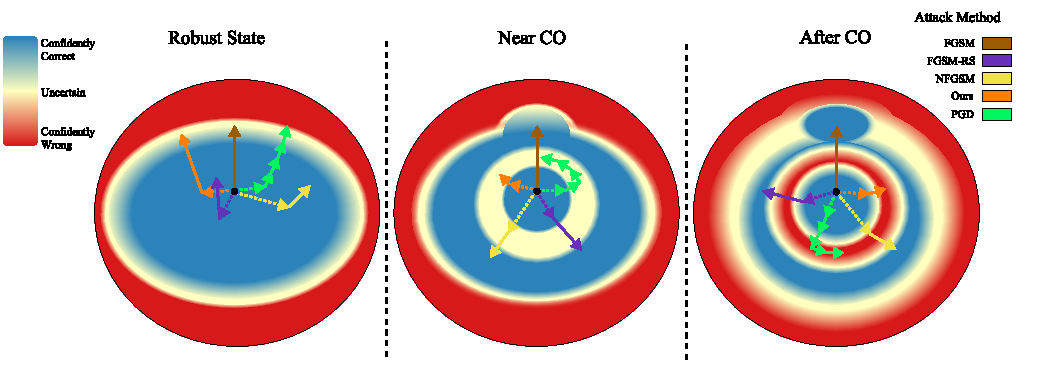
\includegraphics[width=\linewidth,height=.50\paperheight,keepaspectratio]{paper_geometry.pdf}
\caption{پیچش مرز تصمیم و تغییر سطح هزینه؛ بازنشر شکل ۱ مقالهٔ \sora{} \cite{sora2026}.}
\end{figure}
\centering نقطهٔ انتهاییِ کم‌هزینه، نقاط پرهزینهٔ مسیر را پنهان می‌کند.
\note{از چپ به راست توضیح دهید: هندسهٔ اولیه، تغییر پیش از فروپاشی، سپس شکست تک‌گامی. این تصویر تفسیر سازوکار مقاله است و قضیهٔ عمومی دربارهٔ همهٔ شبکه‌ها نیست.}
\end{frame}

% MAIN 09 | 0:55
\begin{frame}{بیش‌برازش اپسیلون؛ حساسیت به اندازهٔ آشفتگی}
% Provenance: supplied paper_epsilon.pdf, published SORA Figure 2;
% original paper sweep, no new measurements or seminar results.
\begin{figure}
\centering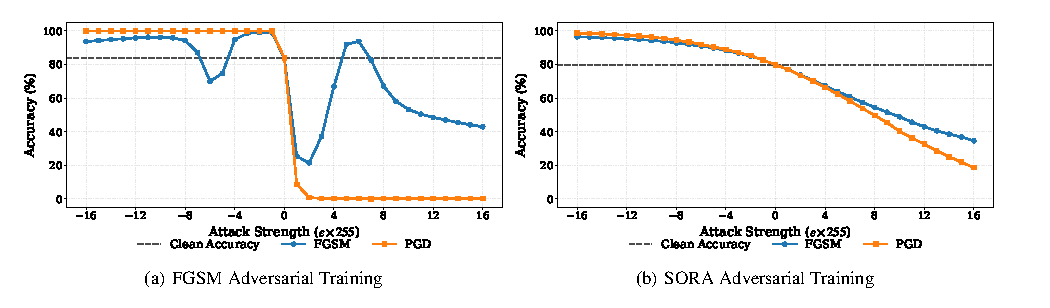
\includegraphics[width=\linewidth,height=.48\paperheight,keepaspectratio]{paper_epsilon.pdf}
\caption{درستی در اندازه‌های مختلف حمله؛ بازنشر شکل ۲ مقالهٔ \sora{} \cite{sora2026}.}
\end{figure}
\begin{itemize}
\item یادگیری در اندازه‌های خاص، محافظت یکنواخت در همسایگی نیست.
\item ضریب منفی محور، حرکت خلاف جهت است؛ شعاع تهدید منفی نیست.
\end{itemize}
\note{نامونوا بودن مربوط به پاسخ یک حملهٔ تقریبی است. بیشینهٔ دقیق هزینه روی مجموعه‌های تودرتو با بزرگ‌شدن شعاع کاهش نمی‌یابد. بیش‌برازش اپسیلون توضیحی برای بخشی از پدیده است، نه شرط لازم و کافی اثبات‌شدهٔ تمام فروپاشی‌ها.}
\end{frame}

% MAIN 10 | 0:45
\begin{frame}{نمونهٔ هم‌آورد غیرعادی؛ نشانه‌ای از عبور از قله}
\[
z=x+\eta,\qquad \ell(z+\delta)<\ell(z)
\]
\begin{itemize}
\item حمله برای افزایش هزینه ساخته شده، ولی در انتها هزینه را کاهش داده است.
\item غیرعادی بودنِ \lr{AAE} دربارهٔ هزینه است؛ الزاماً دربارهٔ درست‌بودن برچسب نیست.
\item جهت شیب می‌تواند پیش از رخ‌دادن این افت هزینه تغییر کند.
\end{itemize}
\takeaway{مقایسهٔ دو شیب می‌تواند اطلاعاتی زودتر از مقایسهٔ دو هزینه بدهد.}
\src{تعریف \lr{AAE}: \cite{lin2023eliminating}؛ انگیزهٔ پایش هندسی: \cite{sora2026}.}
\end{frame}

% MAIN 11 | 0:55
\begin{frame}{هم‌راستایی آشفتگی؛ دو شیبِ در دسترس}
\[
g=\nabla\ell(z),\quad g'=\nabla\ell(z+\delta),\qquad
P=\frac{g^{\mathsf T}g'}{\|g\|_2\|g'\|_2}
\]
\begin{itemize}
\item \pa{} جهت شیب ابتدا و انتهای حمله را مقایسه می‌کند.
\item شیب اول برای حمله و شیب دوم همراه پس‌انتشار روی نمونهٔ هم‌آورد موجود است.
\item مقدار نزدیک یک: حفظ جهت دو شیب؛ به‌تنهایی گواهِ خمیدگی کم نیست.
\end{itemize}
\src{رابطهٔ ۲، صفحهٔ ۵ مقالهٔ \sora{} \cite{sora2026}؛ تعریف برای شیب‌های ناصفر.}
\note{دریافت مشتق ورودی در گذر دوم، حلقهٔ حملهٔ تازه نمی‌خواهد. محاسبات نرم و ضرب داخلی هزینهٔ محدود دارند. محافظت از مخرج صفر در بازتولید باید مشخص شود. در اجرا، شیب دوم نسبت به ورودی نهایی پس از برش گرفته می‌شود.}
\end{frame}

% MAIN 12 | 1:00
\begin{frame}{شواهد هشدار: حدود ۵۰ دسته در یک مسیر مشخص}
% Provenance: supplied paper_pertalign.pdf, SORA Figure 3; timing interpreted
% using paper pp.44--46 / thesis results, NOT a calibrated predictor study.
\begin{figure}
\centering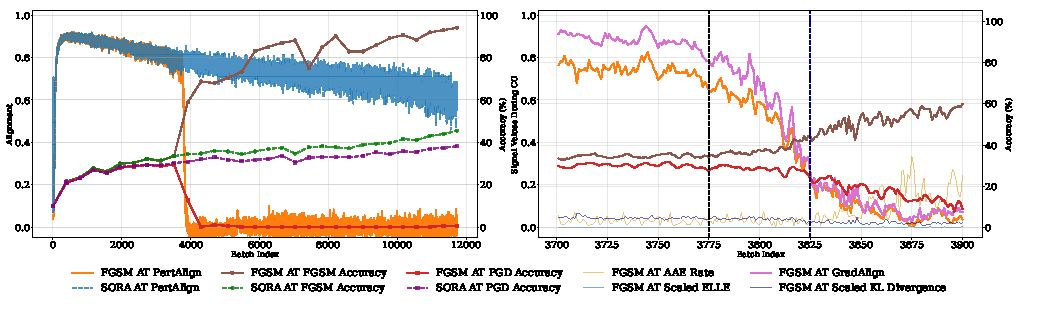
\includegraphics[width=\linewidth,height=.46\paperheight,keepaspectratio]{paper_pertalign.pdf}
\caption{افت هم‌راستایی پیش از جدایی درستی‌ها؛ بازنشر شکل ۳ مقالهٔ \sora{} \cite{sora2026}.}
\end{figure}
\begin{itemize}
\item در مثال \lr{FGSM}: افت حدود دستهٔ $3775$؛ جدایی آشکار حدود $3825$.
\item این فاصله، میانگین عمومی یا مهلت تضمین‌شده نیست؛ آستانه و نرخ هشدار کاذب گزارش نشده‌اند.
\end{itemize}
\note{اعداد خوانش نموداری صفحات ۴۴ تا ۴۶ هستند. گرادالاین نیز زود واکنش می‌دهد و سنجهٔ ELLE با تبدیل مناسب می‌تواند در همان حوالی تغییر کند. مزیت ادعا‌شده ترکیب زمان واکنش و استفاده از شیب‌های موجود است. تبدیل ۵۰ دسته به دوره یا ثانیه بدون مشخصات مسیر مجاز نیست.}
\end{frame}

% MAIN 13 | 1:05
\begin{frame}{رابطهٔ هندسی: بخش عمودِ کنش هسین}
برای $g\ne0$، جهت ثابت $v$ و گام کوچک $\alpha$:
\[
H=\nabla^2\ell(z),\qquad
Q_g=I-\frac{gg^{\mathsf T}}{\|g\|_2^2}
\]
\[
1-P=\frac{\alpha^2}{2\|g\|_2^2}\|Q_gHv\|_2^2+O(\alpha^3)
\]
\begin{itemize}
\item فرض: همواری محلی و هسین محلی لیپشیتس؛ جهت در بسط ثابت است.
\item $P\approx1$ کوچک‌بودن $\|H\|$ را نتیجه نمی‌دهد؛ تغییر موازیِ شیب دیده نمی‌شود.
\end{itemize}
\src{صورت تصویریِ بازنویسی‌شده در فصل هندسه، بر پایهٔ پیوست \lr{A} مقاله \cite{sora2026}.}
\note{مثال شفاهی در صورت نیاز: هسین ام ضربدر همانی و جهت خود شیب، شیب انتهایی را فقط مقیاس می‌کند؛ کسینوس یک می‌ماند، حتی برای ام بزرگ. این رابطه برای جهت علامت هم با همان جهت ثابت معتبر است؛ فرمول خاص جهت خود شیب را نباید به علامت آن منتقل کرد.}
\end{frame}

% MAIN 14 | 1:10
\begin{frame}{بخش دقیق نظری: بهینهٔ اسکالر یک مدل درجه‌دو}
\[
p=\sign(g),\quad q(a)=\ell(z)+ba+\tfrac12ca^2,
\quad b=\|g\|_1>0,\ c=p^{\mathsf T}Hp
\]
\[
\underset{0\leq a\leq A}{\arg\max}\;q(a)=
\begin{cases}
\min\{A,-b/c\},&c<0,\\
A,&c\geq0.
\end{cases}
\]
\begin{itemize}
\item در جهت مقعر، حرکت پس از رأس هزینه را کاهش می‌دهد.
\item این جوابِ دقیقِ مدل اسکالر است؛ سطح واقعی الزاماً درجه‌دو نیست.
\end{itemize}
\src{استخراج فصل روش، بر پایهٔ تحلیل مرتبهٔ دوم مقالهٔ \sora{} \cite{sora2026}.}
\note{برای c نامنفی با b مثبت، مشتق روی نیم‌خط مثبت است و نقطهٔ انتهایی بهینه می‌شود. فقط در حالت c منفی رأس مثبت داریم. فرض g ناصفر را حفظ کنید؛ برای شیب صفر، نسبت‌ها تعریف نظری ندارند.}
\end{frame}

% MAIN 15 | 1:00
\begin{frame}{اطلاعات خمیدگی از همان گام کاوش}
در مدل درجه‌دو، بدون برش و با گام اسکالر $a_{\mathrm{probe}}>0$:
\[
g_{\mathrm{probe}}=g+a_{\mathrm{probe}}Hp,\qquad
r=\frac{p^{\mathsf T}g_{\mathrm{probe}}}{\|g\|_1}
=1+\frac{a_{\mathrm{probe}}c}{b}
\]
\[
r<1\quad\Longrightarrow\quad
a_{\mathrm{quad}}=\min\left\{A,\frac{a_{\mathrm{probe}}}{1-r}\right\}
\]
\begin{itemize}
\item صورت کسر، همان گامی است که شیب دوم با آن اندازه‌گیری شده است.
\item نسبت $r$ با کسینوس \pa{} برابر نیست؛ بزرگی شیب نیز در آن نقش دارد.
\end{itemize}
\src{بازنویسی دقیق فصل روش از استخراج مقالهٔ \sora{} \cite{sora2026}.}
\end{frame}

% MAIN 16 | 1:00
\begin{frame}{قاعدهٔ عملی: کنترل دامنه، الهام‌گرفته از مدل درجه‌دو}
\[
F(u)=\begin{cases}
\min\!\left\{\alpha_{\max},\dfrac{\alpha_0}{1-u}\right\},&u<1,\\
\alpha_{\max},&u\geq1,
\end{cases}
\qquad a_j\sim\mathcal U(0,A_i)
\]
\begin{itemize}
\item $u$ میانگین نماییِ نسبت؛ $A_i$ سقف توزیع گام مؤلفه‌هاست.
\item جایگزینی گام کاوش با $\alpha_0$، همانی دقیقِ اسلاید قبل را تغییر می‌دهد.
\item تصادفی‌سازی مؤلفه‌ای و استفاده از گذشته نیز انتخاب‌های اجرایی‌اند.
\end{itemize}
\src{الگوریتم ۱ مقاله \cite{sora2026}: $\alpha_0=0.02$، $\beta=0.05$، $\alpha_{\max}=2\epsilon$.}
\note{به جای عبارت اندازهٔ گام بهینهٔ هر نمونه از سقف تطبیقی استفاده کنید. در مسیر مؤلفه‌ای، شیب دوم به H diag(a) p وابسته است و لزوماً رابطهٔ کاوش اسکالر را ندارد. موفقیت تجربی این قاعده تضمین بهینگی سراسری نیست.}
\end{frame}

% MAIN 17 | 0:40
\begin{frame}{چرا اصلاح گام می‌تواند مفید باشد؟}
% Provenance: supplied paper_recovery.pdf, SORA Figure 4; original conceptual
% paper illustration, not a new recovery experiment or universal guarantee.
\begin{figure}
\centering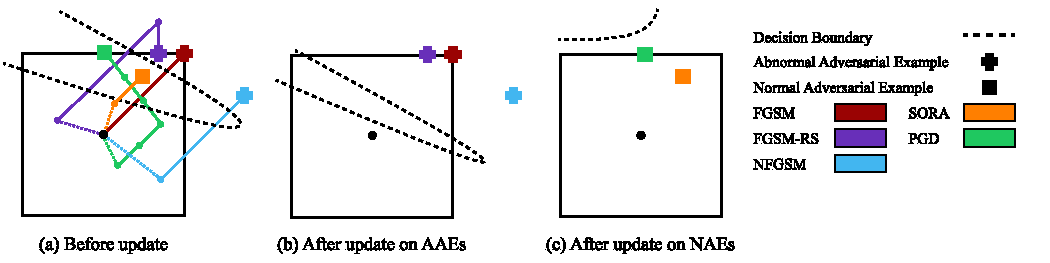
\includegraphics[width=\linewidth,height=.50\paperheight,keepaspectratio]{paper_recovery.pdf}
\caption{تفسیر هندسی اصلاح گام؛ بازنشر شکل ۴ مقالهٔ \sora{} \cite{sora2026}.}
\end{figure}
\centering دسترسی به نقاط پرهزینه می‌تواند آموزش را به ناحیهٔ آسیب‌پذیر بازگرداند.
\note{این شکل تبیین سازوکار است؛ تضمین بازیابی پس از هر فروپاشی نیست. کنترل دامنه تلاش می‌کند از عبور یک‌باره از ناحیهٔ پرهزینه جلوگیری کند.}
\end{frame}

% MAIN 18 | 0:55
\begin{frame}{جریان \sora{}: استفادهٔ دوباره از دو گذر}
% Provenance: NEWLY COMPOSED flow diagram from SORA Algorithm 1 p.6;
% this exact diagram is NOT an original paper/seminar figure.
\begin{figure}
\centering
\begin{latin}
\centering
\begin{tikzpicture}[node distance=5mm,
 stage/.style={draw=sharifblue,rounded corners,fill=sharifblue!5,
   minimum height=12mm,text width=28mm,align=center,font=\small},
 flow/.style={-{Latex[length=2mm]},thick,sharifblue}]
\node[stage] (start) {$z=x+\eta$\\$g=\nabla\ell(z)$};
\node[stage,right=of start] (attack) {$a_j\sim U(0,A_i)$\\$\widetilde x=\Pi_{[0,1]}(z+a\odot p)$};
\node[stage,right=of attack] (train) {$\nabla_{(\widetilde x,\theta)}\ell$\\$g',\ g_\theta$};
\node[stage,right=of train] (control) {$P,\ \bar r_i$\\$A_{i+1}$ \rl{سپس} $u_i$};
\draw[flow] (start)--(attack);
\draw[flow] (attack)--(train);
\draw[flow] (train)--(control);
\draw[flow] (control.south)--++(0,-9mm)-|node[pos=.25,below,font=\small]
  {\rl{آمار گذشته برای دسته‌های بعدی}} (attack.south);
\end{tikzpicture}
\end{latin}
\caption{نمودار تازه‌تدوین‌شده از الگوریتم ۱ مقاله \cite{sora2026}؛ این نمودار در اصل مقاله یا سمینار نیست.}
\end{figure}
\begin{itemize}
\item گذر دوم، هم مشتق وزن‌ها و هم شیب ورودی انتهایی را می‌دهد.
\item \pa{} برای پایش است؛ نسبت $r$ وارد کنترل گام می‌شود.
\end{itemize}
\end{frame}

% MAIN 19 | 1:10
\begin{frame}{شبه‌کد و تأخیر مهمِ ترتیب چاپ‌شده}
% Provenance: newly composed compact Persian restatement of SORA Algorithm 1,
% preserving line 11 before line 12; explicit A1 and batch reduction follow
% thesis method conventions, NOT fully specified by the printed algorithm.
\begingroup\fontsize{12}{16}\selectfont
\begin{enumerate}
\item آغاز: $u_0=0.99$، $A_1=F(u_0)$؛ برای هر دسته، $\eta\sim U([-\epsilon,\epsilon]^d)$.
\item $g=\nabla\ell(x+\eta)$، $p=\sign(g)$؛ جداسازی جهت از گراف حمله.
\item $a_j\sim U(0,A_i)$؛ $\widetilde x=\Pi_{[0,1]^d}(x+\eta+a\odot p)$.
\item دریافت $(g',g_\theta)$؛ به‌روزرسانی وزن‌ها؛ محاسبهٔ $\bar r_i$ از نسبت‌های نمونه‌ای.
\end{enumerate}\endgroup
\[
\boxed{A_{i+1}=F(u_{i-1})}\quad\text{سپس}\quad
u_i=(1-\beta)u_{i-1}+\beta\bar r_i
\]
\textbf{مشاهدهٔ دستهٔ $i$ نخست می‌تواند روی سقفِ دستهٔ $i+2$ اثر بگذارد.}
\src{بازنویسی الگوریتم ۱، صفحهٔ ۶ \cite{sora2026}؛ مقداردهی $A_1$ و میانگین نسبت‌ها قرارداد صریح فصل روش‌اند.}
\note{سطر گام بعد پیش از سطر میانگین نمایی است. این ترتیب را به‌طور خاموش اصلاح نکرده‌ایم. میانگین نسبت نمونه‌ها با نسبت مجموع‌ها یکی نیست و مقاله تجمیع را روشن نکرده است. تأخیر، علاوه بر حافظهٔ میانگین نمایی وجود دارد.}
\end{frame}

% MAIN 20 | 1:00
\begin{frame}{دامنهٔ آموزش با کرهٔ تهدید ارزیابی یکسان نیست}
\[
\widetilde x=\Pi_{[0,1]^d}(x+\eta+a\odot p),\qquad
\|\eta+a\odot p\|_\infty\leq\epsilon+\alpha_{\max}=3\epsilon
\]
\begin{itemize}
\item آموزش: فقط برش پیکسل به $[0,1]$؛ بدون تصویرشدن به کرهٔ $\epsilon$.
\item $3\epsilon$ کرانِ آشفتگی خام است؛ اندازهٔ ثابتِ همهٔ نمونه‌ها نیست.
\item ارزیابی: کرهٔ $\epsilon$ و دامنهٔ پیکسل؛ معمولاً $8/255$، برای \lr{TissueMNIST} برابر $3/255$.
\end{itemize}
\src{الگوریتم ۱ و پیوست \lr{D}، صفحهٔ ۳۱ مقاله \cite{sora2026}.}
\note{در شبه‌کد اصلی، نقطهٔ شیب اول یعنی ایکس به علاوهٔ نویز نیز پیش از محاسبه برش نمی‌خورد. افزودن آن برش یا برش به کره، تغییر روش است. بودجه باید در مقیاس پیکسل پیش از نرمال‌سازی تفسیر شود.}
\end{frame}

% MAIN 21 | 0:45
\begin{frame}{رفتار تطبیقی روی دو دادگان متفاوت است}
% Provenance: supplied paper_stepsize.pdf, SORA Figure 5; original published
% monitoring curves, NOT a newly run experiment or exact-optimum trace.
\begin{figure}
\centering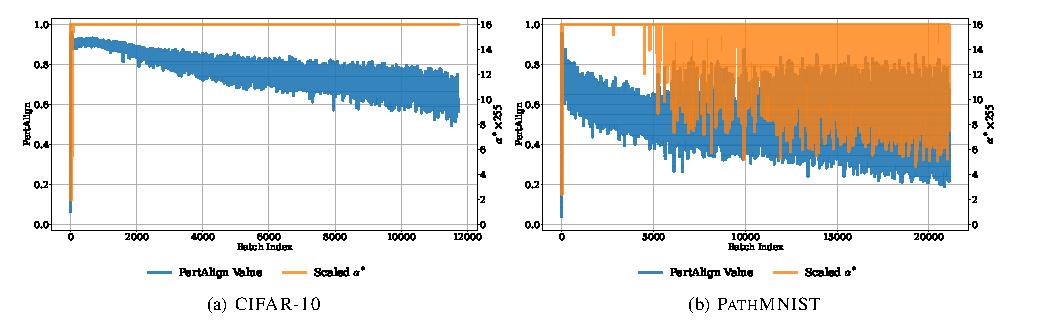
\includegraphics[width=\linewidth,height=.50\paperheight,keepaspectratio]{paper_stepsize.pdf}
\caption{هم‌راستایی و سقف گام؛ بازنشر شکل ۵ مقالهٔ \sora{} \cite{sora2026}.}
\end{figure}
\centering در \lr{CIFAR-10} سقف اغلب فعال است؛ در \lr{PathMNIST} کاهش گام بیشتر رخ می‌دهد.
\end{frame}

% MAIN 22 | 0:55
\begin{frame}{تنظیم و دامنهٔ ارزیابی}
\begin{itemize}
\item دادگان: \lr{CIFAR-10/100}، \lr{TinyImageNet}، \lr{ImageNet-100}، \lr{PathMNIST} و \lr{TissueMNIST}.
\item معماری‌ها: \lr{PreActResNet-18}، \lr{ResNet-18}، \lr{WRN-28-10} و \lr{SENet-18}؛ مدل‌ها جداگانه آموزش می‌بینند.
\item \lr{SGD}: تکانهٔ $0.9$، افت وزن $5\!\times\!10^{-4}$؛ نرخ طبیعی چرخه‌ای، پزشکی کسینوسی.
\end{itemize}
\takeaway{«تنظیم ثابت» یعنی مجموعهٔ نهایی مشترک پس از تنظیم محدود؛ آماده‌سازی داده و همهٔ جزئیات آموزش یکسان نیستند.}
\src{بخش ۶ و پیوست‌های \lr{D, E, M.3} مقاله، صفحات ۳۰ تا ۳۴ و ۶۰ \cite{sora2026}.}
\note{تعمیم در اینجا انتقال تنظیمات میان آموزش‌های جداگانه است، نه آزمودن یک مدل سیفار روی تصاویر پزشکی. سه بذر برای بیشتر آزمایش‌ها گزارش شده؛ ایمیج‌نت صدکلاسه فقط یک اجرا دارد. افزایش داده مطابق دادگان متفاوت است.}
\end{frame}

% MAIN 23 | 1:00
\begin{frame}{نتیجهٔ اصلی؛ دو مسئلهٔ دشوار}
% Provenance: exact selected entries of SORA main Table 1 p.9;
% original table content, translated headings, no new run or mixed reports.
\begin{table}
\centering
\begin{latin}
\centering\fontsize{12}{17}\selectfont\renewcommand{\arraystretch}{1.3}
\begin{tabular}{lrrrr}
\toprule
&\multicolumn{2}{c}{PathMNIST}&\multicolumn{2}{c}{ImageNet-100}\\
\rl{روش}&\rl{پاک}&AA&\rl{پاک}&AA\\
\midrule
FGSM&46.06&0.42&15.94&0.00\\
N-FGSM&74.89&1.65&49.40&15.52\\
AAER&83.54&2.48&48.26&17.18\\
\bfseries SORA&\bfseries85.93&\bfseries32.91&\bfseries57.26&\bfseries18.56\\
\bottomrule
\end{tabular}
\end{latin}
\caption{بازنشر داده‌های جدول ۱، صفحهٔ ۹ مقاله \cite{sora2026}؛ \lr{PreActResNet-18}، $\epsilon=8/255$؛ همهٔ مقادیر درصد.}
\end{table}
\centering بهبود \lr{AA} نسبت به \lr{N-FGSM}: به‌ترتیب $31.26$ و $3.04$ واحد درصد.
\note{جدول ۱ را مستقل بخوانید. نتیجهٔ ایمیج‌نت تک‌اجرایی است؛ اختلاف ۱٫۳۸ واحد درصد با AAER را نمی‌توان معنادار آماری نامید. اینجا عددهای حذف مؤلفه‌ها یا گزارش تجمیعی پیوست وارد نشده‌اند.}
\end{frame}

% MAIN 24 | 0:55
\begin{frame}{تعمیم تنظیمات؛ تصویر کلیِ عملکرد نسبی}
% Provenance: supplied paper_generalization.pdf, SORA Figure 6 p.8;
% normalization described p.47, original paper figure, no new aggregation.
\begin{figure}
\centering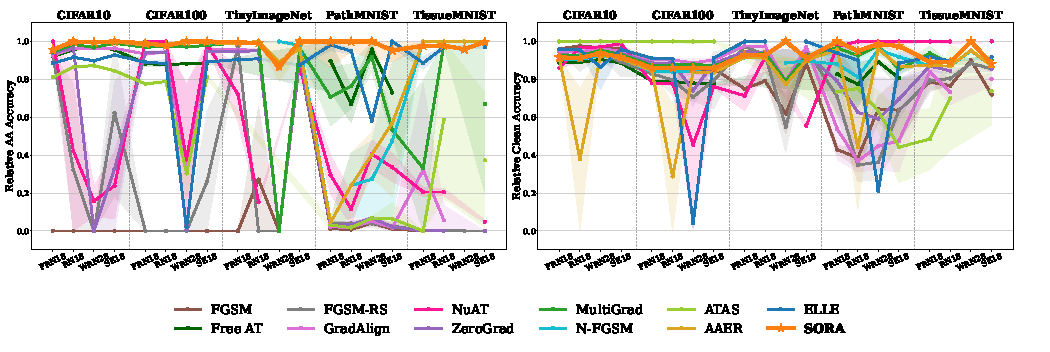
\includegraphics[width=\linewidth,height=.49\paperheight,keepaspectratio]{paper_generalization.pdf}
\caption{بازنشر شکل ۶، صفحهٔ ۸ مقاله \cite{sora2026}؛ نرمال‌سازی نسبت به بهترین مقدار هر مسئله، طبق صفحهٔ ۴۷.}
\end{figure}
\begin{itemize}
\item مقدار نزدیک یک یعنی نزدیکی به بهترین نتیجهٔ همان ستون.
\item مقادیر مطلق و اختلاف‌های کوچک در این نمایش پنهان می‌شوند.
\end{itemize}
\note{بهترین پاک و بهترین هم‌آورد ممکن است متعلق به دو روش متفاوت باشند. نمودار شاهدی دربارهٔ انتقال تنظیم نهایی است و به معنای برتری در تمام خانه‌های جدول‌های تفصیلی نیست.}
\end{frame}

% MAIN 25 | 0:55
\begin{frame}{جدول‌های تفصیلی؛ برتری در همهٔ ستون‌ها برقرار نیست}
% Provenance: NEWLY COMPOSED selected central values from SORA Tables 20
% p.48, 24 p.50, 30 p.53; NOT an original paper/seminar table. +/- omitted.
\begin{table}
\centering
\begin{latin}
\centering\fontsize{12}{15}\selectfont\renewcommand{\arraystretch}{1.1}
\begin{tabular}{llrrr}
\toprule
\rl{دادگان و مدل} & \rl{روش} & \rl{پاک} & PGD-10 & AA\\
\midrule
CIFAR-10 / PreAct-18 & N-FGSM &79.05&48.73&43.95\\
& SORA &79.90&48.64&43.83\\
CIFAR-100 / PreAct-18 & N-FGSM &53.43&26.25&21.75\\
& SORA &54.74&26.12&21.56\\
TinyImageNet / WRN-28-10 & N-FGSM &48.47&21.21&\bfseries16.58\\
& SORA &54.59&18.73&14.31\\
\bottomrule
\end{tabular}
\end{latin}
\caption{چینش تازه از جدول‌های ۲۰، ۲۴ و ۳۰، صفحات ۴۸، ۵۰ و ۵۳ مقاله \cite{sora2026}؛ فقط مقادیر مرکزی درصدی، با حذف $\pm$؛ جدول اصلی مقاله نیست.}
\end{table}
\centering برداشت: بده‌بستان پاک، ستبر و هزینه؛ رتبه‌بندی به مسئله وابسته است.
\end{frame}

% MAIN 26 | 0:55
\begin{frame}{حذف مؤلفه‌ها؛ گزارش مستقلِ \lr{PGD-10}}
% Provenance: exact SORA main Table 2 p.9, PathMNIST/PreActResNet-18;
% original ablation content, NOT Table 1 AA or new experiments.
\begin{table}
\centering
\begin{latin}
\centering\fontsize{12}{17}\selectfont\renewcommand{\arraystretch}{1.3}
\begin{tabular}{lrrr}
\toprule
\rl{تنظیم} & \rl{پاک} & FGSM & PGD-10\\
\midrule
SORA (\rl{پایه})&84.69&57.51&45.56\\
\rl{بدون نمونه‌گیری تصادفی}&85.67&58.89&45.35\\
\rl{برش اندازه گام}&86.82&52.02&34.08\\
\rl{بدون گام تطبیقی}&89.93&28.30&17.23\\
\bottomrule
\end{tabular}
\end{latin}
\caption{جدول ۲، صفحهٔ ۹ مقاله \cite{sora2026}؛ \lr{PathMNIST/PreActResNet-18}، درصد؛ مستقل از گزارش اصلی \lr{AA}.}
\end{table}
\centering حذف سازگاری گام افت بزرگی دارد؛ افت $0.21$ با حذف نمونه‌گیری، به‌تنهایی شاهد معناداری آماری نیست.
\note{نام اصلی سطر آخر در مقاله Without Optimal Step-Size است و در اینجا بدون گام تطبیقی ترجمه شده است؛ ادعای تازهٔ بهینگی دقیق الگوریتم نیست. پاک پایه ۸۴٫۶۹ و معیار ۴۵٫۵۶ از همین آزمایش‌اند. جدول عدم قطعیت این مقایسه را مشخص نکرده است.}
\end{frame}

% MAIN 27 | 0:55
\begin{frame}{کارایی؛ زمان و حافظه در یک تنظیم مشخص}
% Provenance: supplied paper_efficiency.pdf, SORA Figure 7 p.8;
% protocol p.59: PathMNIST/PreAct-18, 30 epochs, RTX4090, training loop only.
\begin{figure}
\centering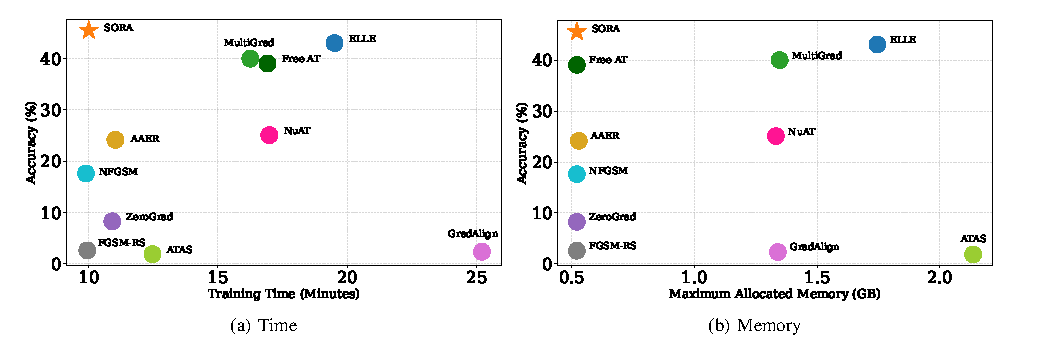
\includegraphics[width=\linewidth,height=.54\paperheight,keepaspectratio]{paper_efficiency.pdf}
\caption{بازنشر شکل ۷، صفحهٔ ۸ مقاله \cite{sora2026}؛ \lr{PathMNIST/PreActResNet-18}، ۳۰ دوره، \lr{RTX 4090}؛ درستی: \lr{PGD-10}.}
\end{figure}
\note{طبق جدول ۱۹ صفحهٔ ۴۸، سورا دو گذر پیشرو و دو پسرو دارد و PGD-10 یازده گذر از هر نوع. نسبت گذرها شتاب واقعی نیست. طبق صفحهٔ ۵۹، زمان شکل فقط حلقهٔ آموزش است؛ بدون ذخیره، بارگذاری و جست‌وجوی تنظیمات. از نمودار زمان دقیق تازه استخراج نکنید. محاسبهٔ ضرب داخلی و نگهداری شیب‌ها صفر نیست. نبود نتیجهٔ ATAS روی TinyImageNet به محدودیت حافظه مربوط است و نباید صفر درستی تعبیر شود.}
\end{frame}

% MAIN 28 | 0:55
\begin{frame}{حدود شواهد و نکات قابل دفاع}
\begin{itemize}
\item هشدار: مشاهدهٔ تقدم زمانی داریم؛ پیش‌بین واسنجی‌شده و نرخ هشدار کاذب نداریم.
\item نظریه: تحلیل محلی و جهت‌وابسته است؛ تصادفی‌سازی، برش و تأخیر فاصله‌ای با مدل دقیق دارند.
\item ارزیابی: \lr{ImageNet-100} تک‌اجرایی است؛ جزئیات کامل حمله‌ها و رابطهٔ بعضی گزارش‌ها روشن نیست.
\end{itemize}
\src{فصل‌های نتایج و جمع‌بندی و پیوست پایان‌نامه؛ پیوست‌های \lr{J, M} مقاله \cite{sora2026}.}
\note{اعداد متن و پیوست را اصلاح یا ادغام نکرده‌ایم. نتایج پزشکی دربارهٔ دسته‌بندی تحت آشفتگی عددی‌اند و ادعای ایمنی بالینی ندارند. آموزش چندگامی همچنان می‌تواند ستبری بیشتری داشته باشد.}
\end{frame}

% MAIN 29 | 0:50
\begin{frame}{دستاورد؛ اتصال پایش هندسی به اصلاح آموزش}
\begin{enumerate}
\item تفسیر بیش‌برازش اپسیلون: اهمیت پوشش اندازه‌ها و جهت‌های متنوع آشفتگی.
\item \pa: پایش تغییر جهت شیب با استفاده از محاسبات موجود و تفسیر هندسی محلی.
\item \sora: کنترل سقف توزیع گام با اطلاعات دو شیب؛ بده‌بستان رقابتی در دامنهٔ ارزیابی‌شده.
\end{enumerate}
\src{دستاوردهای پژوهش مشترک \cite{sora2026}؛ سهم این ارائه، روایت و تحلیل مستند فصل‌های کامل‌شدهٔ پایان‌نامه است.}
\note{دستاوردها را به مقالهٔ مشترک نسبت دهید. ترتیب نویسندگان مبنایی برای نسبت‌دادن بخش خاصی به یک فرد نیست. نتیجهٔ اصلی، امکان استفادهٔ کم‌هزینه از هندسهٔ موجود در آموزش است.}
\end{frame}

% MAIN 30 | 0:50
\begin{frame}{ادامهٔ پژوهش؛ از نشانه تا پیش‌بین قابل سنجش}
\begin{itemize}
\item تعریف مستقل رویداد فروپاشی، تعیین آستانه روی اعتبارسنجی و سنجش هشدار کاذب و پیش‌آگاهی در چند اجرا.
\item کنترل نمونه‌ای یا گروهی برای دادگان نامتوازن؛ سنجش سود در برابر نوسان و هزینه.
\item جداسازی اثر دامنه، تنوع و تطبیق با بودجهٔ محاسباتی و دامنهٔ آموزش یکسان.
\end{itemize}
\takeaway{دو شیبِ موجود می‌توانند هم نشانهٔ هشدار و هم مبنای اصلاح گام باشند؛ ارزیابی مستقلِ ستبری همچنان ضروری است.}
\src{مسیرهای پیشنهادی فصل جمع‌بندی؛ محدودیت‌های مطالعهٔ مشترک \cite{sora2026}.}
\note{این موارد برنامهٔ آینده‌اند و به‌عنوان آزمایش انجام‌شده ارائه نمی‌شوند. در حدود ۲۷ دقیقه پایان دهید؛ اسلایدهای بعد برای بحث فنی و پرسش‌ها هستند.}
\end{frame}

\appendix
% Backups have B labels; the main denominator remains 30.
\setbeamertemplate{footline}{\hfill{\persiansans\fontsize{9}{11}\selectfont
پشتیبان \lr{B\insertframenumber}\hspace{6mm}}\vspace{2mm}}

% BACKUP 01: appendix distinction is confined to backup material.
\begin{frame}{پشتیبان: منشأ گزارش‌ها و اختلاف حل‌نشده}
\begin{itemize}
\item جدول اصلی ۱، صفحهٔ ۹: \lr{PathMNIST}، پاک $85.93$ و \lr{AA} برابر $32.91$.
\item جدول حذف مؤلفه‌های ۲، صفحهٔ ۹: پاک $84.69$ و \lr{PGD-10} برابر $45.56$؛ معیار مستقل.
\item جدول ۳۲، صفحهٔ ۵۳: پاک $84.88\pm0.99$ و \lr{AA} برابر $35.54\pm1.55$؛ گزارش مستقلِ پیوست.
\end{itemize}
\src{همه متعلق به \lr{PathMNIST/PreActResNet-18} در مقاله‌اند \cite{sora2026}؛ رابطهٔ دقیق اجراها روشن نیست. اعداد ادغام یا میانگین‌گیری نشده‌اند.}
\note{این تفاوت به صورت یادداشت پشتیبان حفظ شده است. بدون فرادادهٔ بذر، نقطهٔ کنترل و تنظیم دقیق، یکی را تصحیح دیگری نمی‌نامیم. علامت مثبت‌ومنفی عین گزارش منبع است و فاصلهٔ اطمینان تازه‌ای ساخته نشده است.}
\end{frame}

% BACKUP 02
\begin{frame}{پشتیبان: بازتولید و هزینهٔ ساختاری}
% Provenance: newly composed selection from SORA Table 19 p.48; exact
% pass counts, NOT original paper/seminar table or hardware measurements.
\begin{table}
\centering
\begin{latin}
\centering\fontsize{12}{16}\selectfont
\begin{tabular}{lrr}
\toprule \rl{روش}&\rl{گذر پیشرو}&\rl{گذر پسرو}\\\midrule
FGSM-RS / SORA&2&2\\
GradAlign / ELLE&3&2\\
PGD-2&3&3\\
PGD-10&11&11\\
TRADES&12&11\\\bottomrule
\end{tabular}
\end{latin}
\caption{گزینش و چینش تازه از جدول ۱۹، صفحهٔ ۴۸ مقاله \cite{sora2026}؛ واحد: هر دسته؛ این جدول عین جدول اصلی نیست.}
\end{table}
\begin{itemize}
\item لازم برای بازتولید: بذر، نقطهٔ کنترل، نسخه و تنظیم \lr{AA}، گام و بازآغازهای حمله.
\item تجمیع نسبت‌ها، مخرج صفر، سقف آغاز و ترتیب \lr{EMA} باید صریح ثبت شوند.
\end{itemize}
\end{frame}

% BACKUP 03
\begin{frame}{واژه‌نامهٔ کوتاه: مسئله و ارزیابی}
% Provenance: newly composed glossary table from thesis dictionary and
% paper terminology; NOT an original paper/seminar table or experiment.
\begin{table}
\centering\renewcommand{\arraystretch}{1.3}
\begin{tabular}{rl}
\toprule
فارسی & \lr{English}\\\midrule
هم‌آورد & \lr{Adversarial}\\
آشفتگی & \lr{Perturbation}\\
دادگان & \lr{Dataset}\\
درستی & \lr{Accuracy}\\
ستبری & \lr{Robustness}\\
بیش‌برازش فاجعه‌بار & \lr{Catastrophic Overfitting (CO)}\\
\bottomrule
\end{tabular}
\caption{واژه‌نامهٔ تازه‌تدوین‌شده مطابق واژه‌گزینی پایان‌نامه و اصطلاحات مقاله \cite{sora2026}؛ جدول اصلی مقاله نیست.}
\end{table}
\end{frame}

% BACKUP 04
\begin{frame}{واژه‌نامهٔ کوتاه: هندسه و روش}
% Provenance: newly composed glossary table from thesis dictionary and
% SORA terminology; NOT an original paper/seminar table or experiment.
\begin{table}
\centering\renewcommand{\arraystretch}{1.3}
\begin{tabular}{rl}
\toprule
فارسی & \lr{English}\\\midrule
شیب & \lr{Gradient}\\
خمیدگی & \lr{Curvature}\\
هزینه & \lr{Loss}\\
هم‌راستایی آشفتگی & \lr{Perturbation Alignment (PertAlign)}\\
نمونهٔ هم‌آورد غیرعادی & \lr{Abnormal Adversarial Example (AAE)}\\
میانگین نمایی & \lr{Exponential Moving Average (EMA)}\\
\bottomrule
\end{tabular}
\caption{واژه‌نامهٔ تازه‌تدوین‌شده از اصطلاحات مقاله \cite{sora2026} و واژه‌گزینی پایان‌نامه؛ جدول اصلی مقاله نیست.}
\end{table}
\end{frame}

% BACKUP 05 onward: automatic continuation, normally about three pages.
\begin{frame}[allowframebreaks]{منابع منتخب}
\begin{latin}
\fontsize{10}{12}\selectfont
\bibliographystyle{unsrt}
\bibliography{defense_references}
\end{latin}
\end{frame}
\end{document}
